%removes listed appendices from toc
%\addtocontents{toc}{\protect\setcounter{tocdepth}{0}}

\chapter*{Appendices}
\thispagestyle{headings}

%\addtocontents{toc}{\protect\setcounter{tocdepth}{2}}
\listofappendices{}
\clearpage

%removes listed appendices from toc
%\addtocontents{toc}{\protect\setcounter{tocdepth}{0}}

\renewcommand\thesection{\Alph{section}}

\section{Introduction poster}\appcaption{Appendix A ~ Introduction poster}
\label{introposter}
This poster was given to all units of KVPS as an introduce to the experimentation. 
\bigskip

\begin{figure}[ht]
   %\begin{center}
    %    \subfigure{
           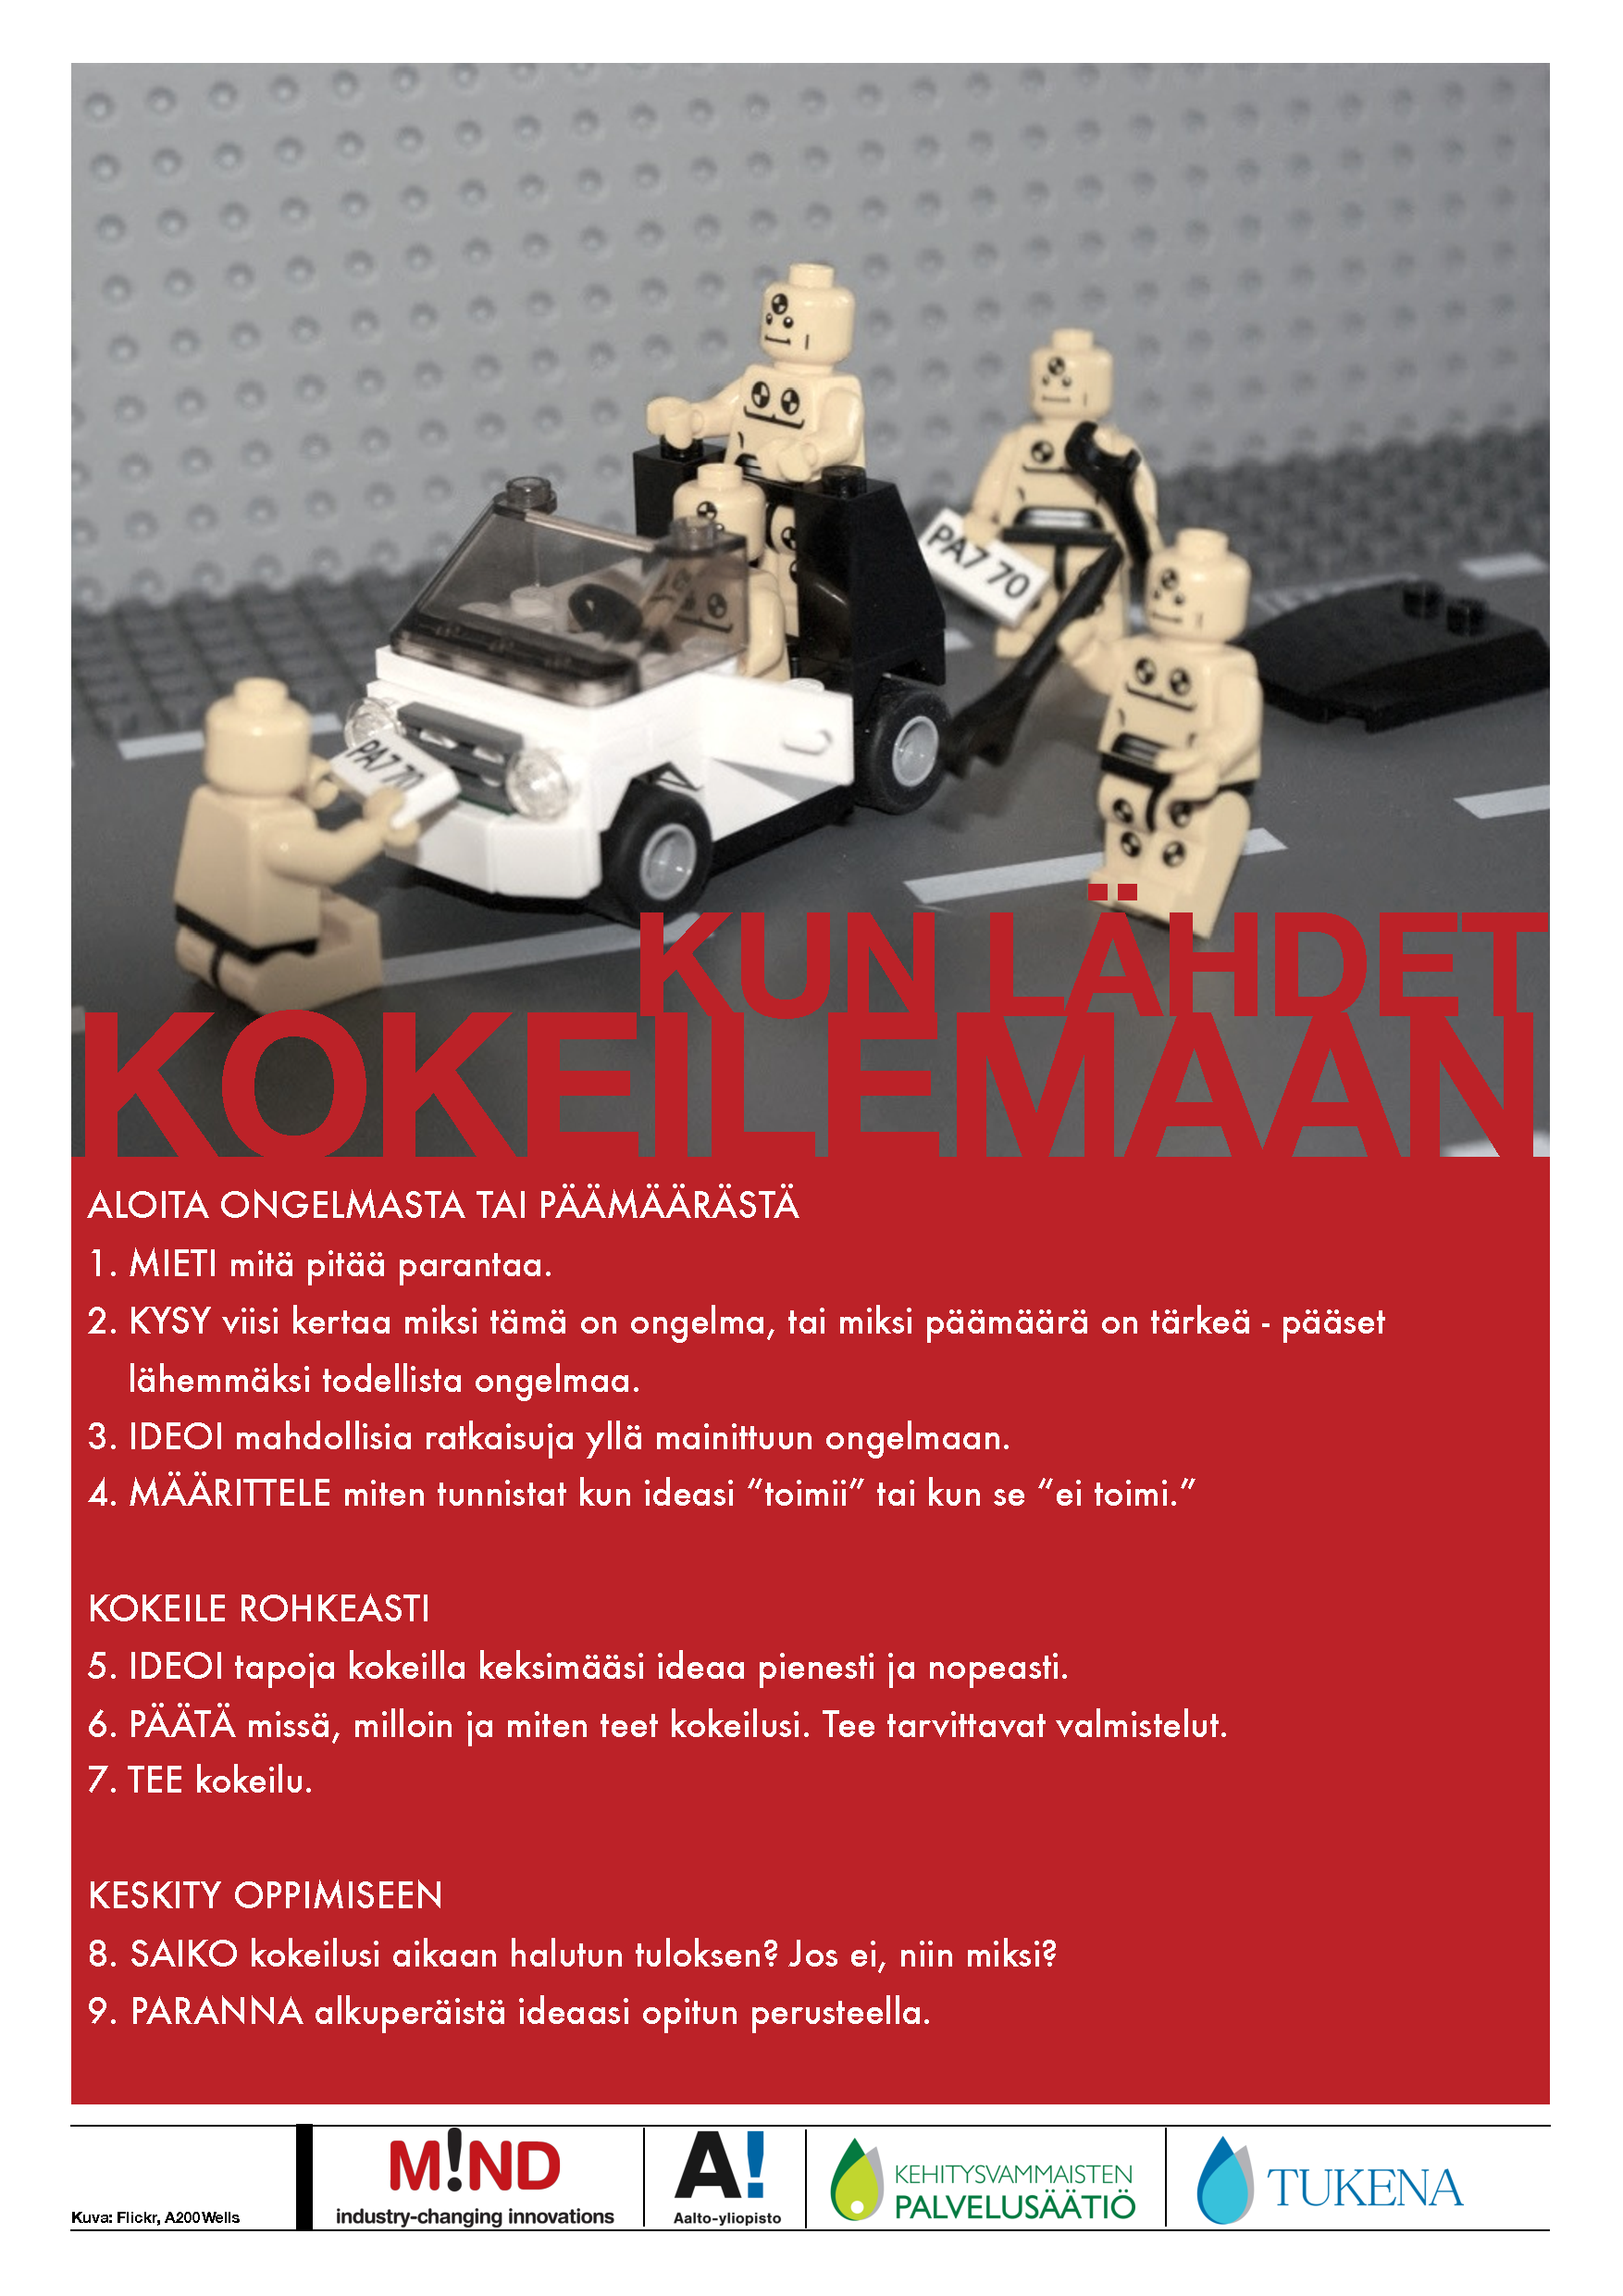
\includegraphics[width=0.83\textwidth]{juliste.pdf}
  %    }
   % \end{center}
\end{figure}

% start next appendix on new page
\clearpage
\section{Idea formula}\appcaption{Appendix B ~ Idea formula}
\label{ideaformula}
Participants of the experimentation challenge were asked to report experiments via this formula.  
\bigskip

\begin{figure}[ht]
   %\begin{center}
    %    \subfigure{
           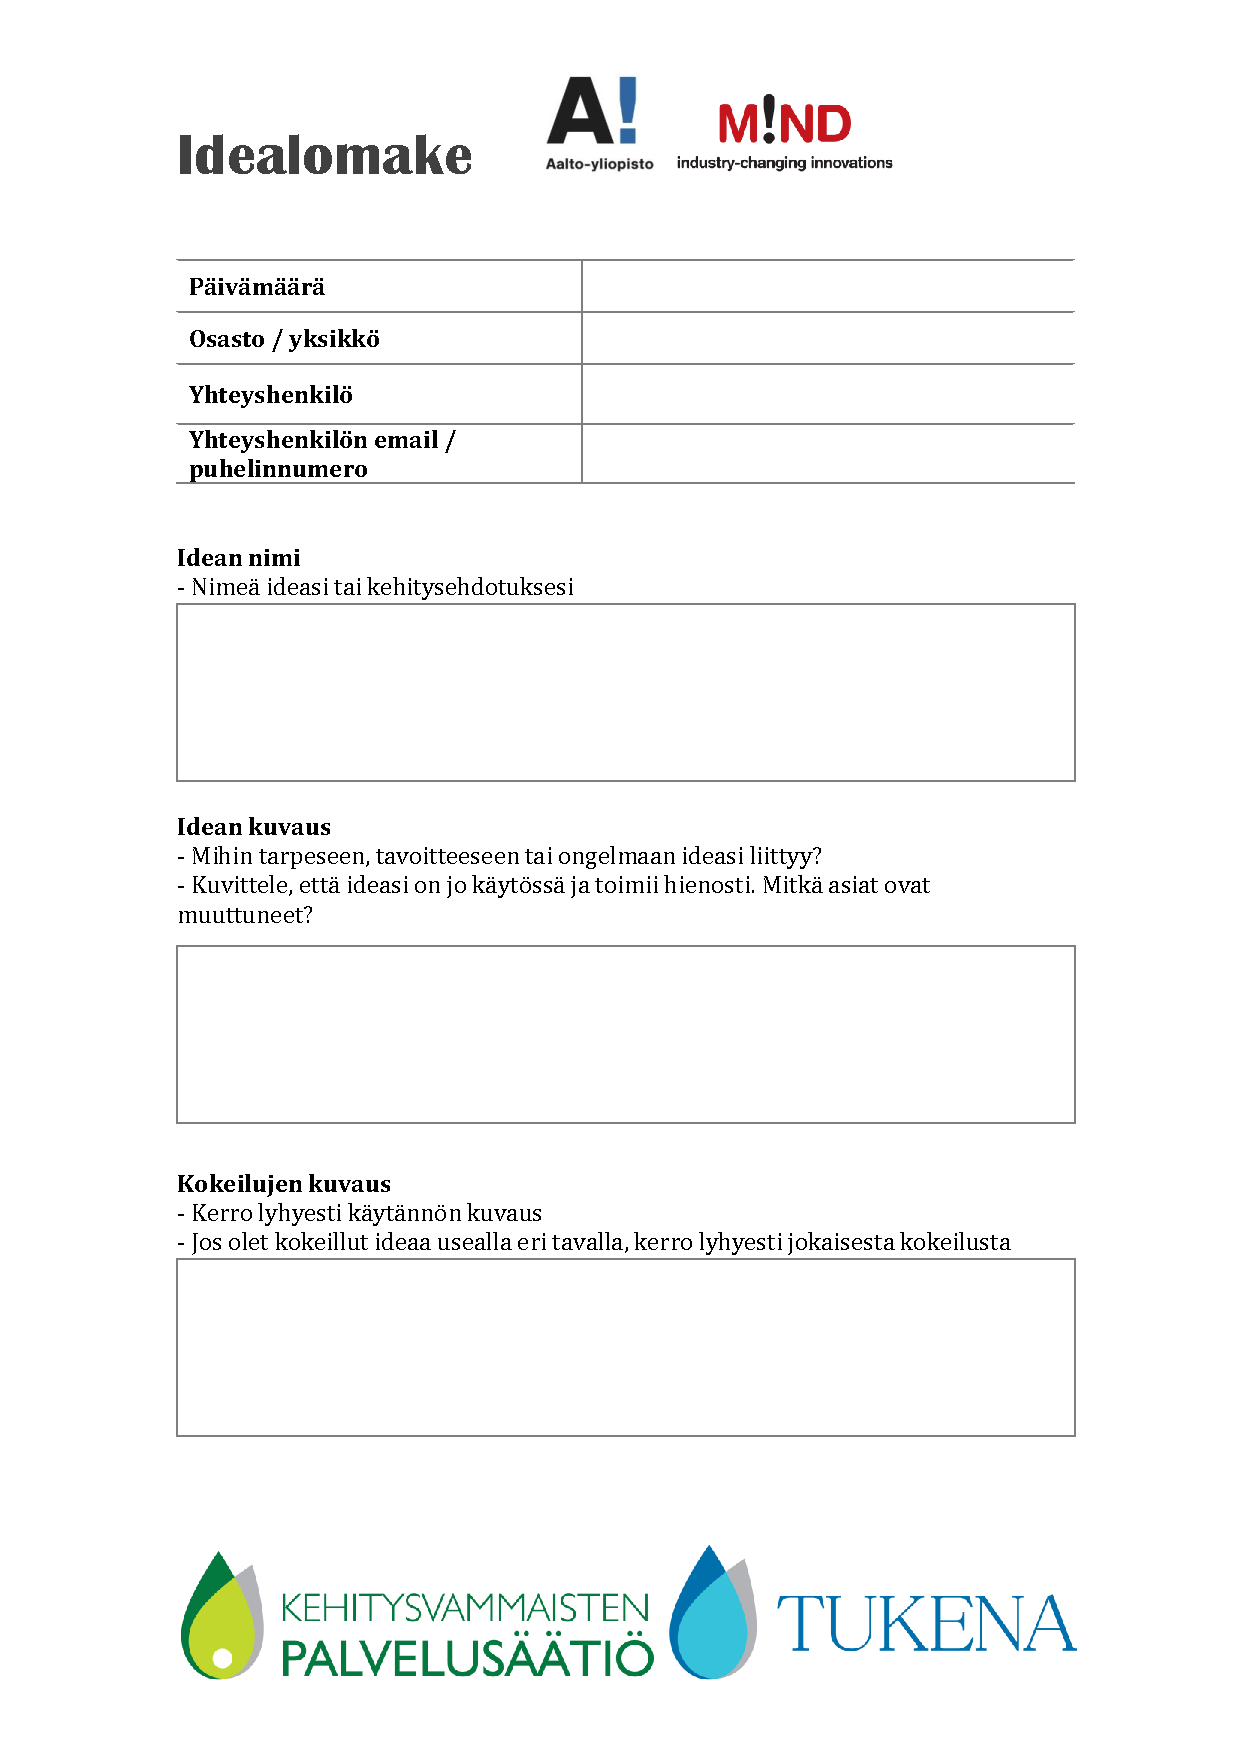
\includegraphics[width=0.83\textwidth]{idealomake.pdf}
  %    }
   % \end{center}
\end{figure}

% start next appendix on new page
\clearpage

\section{Interview questions}\appcaption{Appendix C ~ Interview questions}
\label{haastisrunko}
The interview questions are presented below.
\bigskip

\noindent\emph{Background}
\vspace{-3mm} 
\begin{list}{*}{}
\setlength{\itemsep}{-3pt}
 \item Work description, and how long has the interviewee been in the position?
\end{list}

\noindent \emph{Know-how}
\vspace{-3mm} 
\begin{list}{*}{}
\setlength{\itemsep}{-3pt}
 \item What experiments did you do during the experimentation challenge?
 \item What idea did you work on further?
 \item How did you progress? What did you do?
 \item Did you develop the idea and conducted an experiment alone or together with colleagues? Did this deviate from your conventional way of working? 
\newline
 \item What did you find easy? (What made it easy?)
 \item What did you find difficult? (What made it difficult?)
 \item Did something surprising or unexpected happen?
 \item How did you act in this situation?
 \item What do you personally consider as critical incidents during the experimentation challenge ? eg. What excited you or discouraged?
 \item Where do you think you succeeded? (Why?)
 \item What made an experiment successful? How do you know that an experiment was successful?
 \item What affected to the success of the experiment? What were the conditions?
 \item What went wrong from your perspective? Where did you consider failing? (Why?) 
 \item What made an experiment unsuccessful? 
 \item What affected or caused an experiment to fail? 
 \item Can you describe some idea that you experimented during the experimentation challenge. 
 \item How would you continue developing this idea?
 \item What would you do this time differently than in the first experiment?
 
\end{list}

\noindent\emph{Supporting structures and practices}
\vspace{-3mm} 
\begin{list}{*}{}
\setlength{\itemsep}{-3pt}
    \item How did the experimentation challenge differ from the conventional way of improving ideas?
    \item Have you developed through experimenting before? Is it part of daily routine?
    \item How did experiments affect normal working day and routines?
    \item To whom did you tell about experiments?
    \item How did you document the experiments?
    \item How do you collect feedback from experiments?
    \medskip
\end{list}

\noindent\emph{Climate}
\vspace{-3mm} 
\begin{list}{*}{}
\setlength{\itemsep}{-3pt}
    \item How was the climate of your work unit during the experimentation challenge?
    \item What affected?
    \item Were everybody equally involved?
    \item Did everybody speak up about their ideas? 
    \item Were there conflicts? What were the effects of conflicts?
    \item What kind of support did you get in experimenting from your organisation/your colleagues? 
    \item What kind of support you would have wished?
    \item Is there some specific thing preventing experimenting generally in your work?
    \item What usually happens after telling out an idea? (Do you get support and encouragement and start acting?)
    \item How failed experiments are dealt with in your team? 
\end{list}

\noindent\emph{Leadership behaviour}
\vspace{-3mm} 
\begin{list}{*}{}
\setlength{\itemsep}{-3pt}
    \item How immediate superiors react on new ideas and experimenting?
    \item Is time allocated for ideating and experimenting in your work?
    \end{list}
    
\noindent\emph{Managing experimentation}
\vspace{-3mm} 
\begin{list}{*}{}
\setlength{\itemsep}{-3pt}
     \item  Do you feel that through experimenting you have more autonomy and you can affect better on your own work? Is experimenting one way to affect your work and improve it? 
    \item During the experimentation challenge, did you get more ideas than usually? How did they emerge?
    
\end{list}

\noindent\emph{Psychological factors}
\vspace{-3mm} 
\begin{list}{*}{}
\setlength{\itemsep}{-3pt}
\item What kinds of emotions rose during experimenting? (Did you for instance feel frustrated, insecure etc.)
\item How did it feel to tell an idea out loud among a team? (Do you get support or was your idea refected?)
\item How do you face a failed or unfinished experiment? (If there were any experiments like that)
\item What did you get from the experience of experimentation challenge?
\item What kind of factors brought good feeling? 
\item What kind of factors brought you down or caused anxiety somehow? 

\item How the amount and quality of feedback differs from when developing through experimenting?
\item How do you consider feedback? (Does it encourage to develop an idea further? Did it bring you down?)
\item  How does experimenting affect your own learning and developing your work? 
\end{list}

\noindent\emph{Wrap-up} 
\vspace{-3mm} 
\begin{list}{*}{}
\setlength{\itemsep}{-3pt}
\item Do you have any questions or comments?
\end{list}

% manual page-ref to last page of appendices
\label{appendices-end}